\documentclass[a4paper]{article}
%\usepackage{fourier-otf}
\usepackage[utf8]{inputenc}
\usepackage{graphicx}
\usepackage{algorithm}
\usepackage{algpseudocode}
\usepackage{multirow}
\usepackage{float}
\usepackage{lipsum}
\usepackage{scrextend}
\usepackage{biblatex}
\addbibresource{bibliography.bib}
\usepackage{listings}
\usepackage{amsmath}
\usepackage{amsfonts}
%\usepackage[square,sort,comma,numbers]{natbib}
\newtheorem{theorem}{Theorem}[section]
\usepackage{color}
\usepackage{makeidx}
\usepackage{titlepic}
\definecolor{mygreen}{rgb}{0,0.6,0}
\definecolor{mygray}{rgb}{0.5,0.5,0.5}
\definecolor{mymauve}{rgb}{0.58,0,0.82}
\lstset{ %
	backgroundcolor=\color{white},   % choose the background color
	basicstyle=\footnotesize,        % size of fonts used for the code
	breaklines=true,                 % automatic line breaking only at whitespace
	captionpos=b,                    % sets the caption-position to bottom
	commentstyle=\color{mygreen},    % comment style
	escapeinside={\%*}{*)},          % if you want to add LaTeX within your code
	keywordstyle=\color{blue},       % keyword style
	stringstyle=\color{mymauve},     % string literal style
}
\usepackage{hyperref}
\hypersetup{
  colorlinks   = true,    % Colours links instead of ugly boxes
  urlcolor     = black,    % Colour for external hyperlinks
  linkcolor    = black,    % Colour of internal links
  citecolor    = black      % Colour of citations
}
%\title{First chapter}

%\author{F.Bernardi}

%\protect\\ 

\newcommand{\myName}{Fabrizio Bernardi}
\newcommand{\myTitle}{Modeling and data analysis of the calcium activity in somatostatin interneurons from in vivo imaging on mice }
\newcommand{\myDegree}{Programme: \protect\\ \textit{Mathematical Engineering}}
\newcommand{\myCycle}{XXXI cycle}
\newcommand{\myDepartment}{Department of Mathematics}
\newcommand{\myUni}{Politecnico di Milano}
\newcommand{\myYear}{2022}
\newcommand{\myTime}{01 Jan \myYear}

\pdfbookmark{Cover}{cover}

\begin{document}
	
	
	
\section{Interbrain data analysis: one-to-one task}


\subsection{Description of the task and data normalization}

\begin{figure}[H]
	\begin{center}
		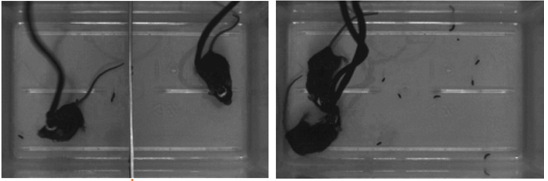
\includegraphics[scale=.85]{one-one.png} 
	\end{center} 
	\caption{\textit{Scheme of the one-to-one task. Left: situation of the pre-test and post-test phase. Right: test phase.}}
	
\end{figure}

In the one-to-one task, two mice are free to interact in an open arena, while the activity of somatostatine-expressing neurons in the anterior cingulate cortex is been recorded through microendoscopic calcium imaging. The task consists in three phases:

\begin{enumerate}
	\item \textbf{Pre-test}. The mice are kept separate by a dark partition, which block their view but still allow them to sniff each other.\\
	$\longrightarrow$ \textit{Duration}: $10$ minutes
	
	\item \textbf{Test}. The mice are free to interact in the arena.\\
	$\longrightarrow$ \textit{Duration}: $15$ minutes
	
	\item \textbf{Post-test}. As in the pre-test, after the test the mice are separated by the same partition.
	$\longrightarrow$ \textit{Duration}: $10$ minutes
\end{enumerate}

In contrast with the emotion discrimination task, discussed in the previous chapter, now there are only two mice which have not been subjected to emotional manipulation. Therefore, the aim of this task is to investigate neural activity and synchronization in a \textit{standard} setting, following the work in [Kingsbury], but with a different neuronal target. Other types of data available are:

\begin{itemize}
	\item The time instants in which reciprocal sniffing is present between the two mice, during the test
	\item The posotion of the micee during pre-test and post-test phases is recorded. From this, two types of zones have been labeled: one near the partition, one far from it, in order to investigate wheter, despite the presence of the partition, the proximity of the two mice could result in a difference in some of the quantities of intrest.
	
	\item Spatial data of the neurons in the ROI are present as in the case pof the emotion discrimination task
\end{itemize}

As for the normalization of the dataset, the same apporach of the previous chapter has been adopted in the one-to-one task as well, namely a z-score normalization performed on the baseline activity of neurons.
\end{document}
